\documentclass[14pt,a4paper]{article}
\usepackage{mathtools}
\usepackage{amsmath}
\setcounter{MaxMatrixCols}{20}
\usepackage{mathrsfs}
\usepackage{setspace}
\usepackage{amsfonts}
\usepackage{geometry}
\geometry{a4paper, total = {210mm,297mm},left=35mm, right=25mm,top=25mm,bottom=25mm}
\usepackage{xcolor}
\usepackage{mcode}
\usepackage{listings}
\lstset{basicstyle = \fontsize{11}{12} \selectfont\ttfamily}
\usepackage{graphicx}


%Begin document - Numerical Analysis - Homework 3

\begin{document}
\label{cover}
\begin{center}
	\vspace*{3cm}
	\large{\textbf{MATH/CS 5466 NUMERICAL ANALYSIS \\ Homework 3}}
	\vfill
	\textbf{Luan Cong Doan} \\ luandoan@vt.edu
	%\vfill
%	Department of Mechanical Engineering \\ Virginia Polytechnic Institute and State University
	\vfill
	\today
\end{center}
\pagebreak

\label{Answer Sheet - Numerical Homework 3}
\doublespacing

\label{Problem 1}
\large\textbf{Problem 1.} Consider the approximation to $f(x) = \sqrt{x}$ for $x \in [0,1]$:
\begin{enumerate}
	\label{1a}
	\item Construct the interpolant $p_1 \in \mathcal{P}_1$ to $f(x)= \sqrt{x}$ using the interpolation points $x_0 = 1/3$ and $x_1 = 1/3$ and produce a plot of the error $\sqrt{x} -p_1(x)$. Identify three points (call them $\tilde{x}_0, \tilde{x}_1, \tilde{x}_2$ in this case) at which the error $f(x) - p_1(x)$ oscillates sign. Apply \textbf{\textit{de la Valee Poussin}}'s theorem to obtain a lower bound on the error $\|f-p_*\|_{\infty}$ in the minimax approximation $p_* \in \mathcal{P}_1$ to $f$ on $[0,1]$.
	
	
	Apply Newton basis for the interpolating polynomial, we have:\\
	\hspace*{2cm} $p_1(x) = p_0(x) + c_1q_1(x)$\\
	with: $p_0(x)= f(x_0) \Rightarrow p_0(x) = \sqrt{\dfrac{1}{3}}$ \\
	\hspace*{1.1cm} $c_1 = \dfrac{f(x_1) - f(x_0)}{x_1 - x_0} = \dfrac{\sqrt{\dfrac{2}{3}} - \sqrt{\dfrac{1}{3}}}{\dfrac{2}{3} - \dfrac{1}{3}} = \sqrt{3}(\sqrt{2} -1)$\\
	\hspace*{1.1cm} $ q_1 = x - x_0 = x - \dfrac{1}{3}$;\\
	$ \Rightarrow p_1(x)= \sqrt{\dfrac{1}{3}} + \sqrt{3}(\sqrt{2} -1)(x - \dfrac{1}{3}) = \sqrt{3}(\sqrt{2} -1)x + \dfrac{2 - \sqrt{2}}{\sqrt{3}}$\\
	
	Plot the error $\sqrt{x} - p_1(x)$ over $[0,1]$:
	\begin{figure}[htp]
		\centering
		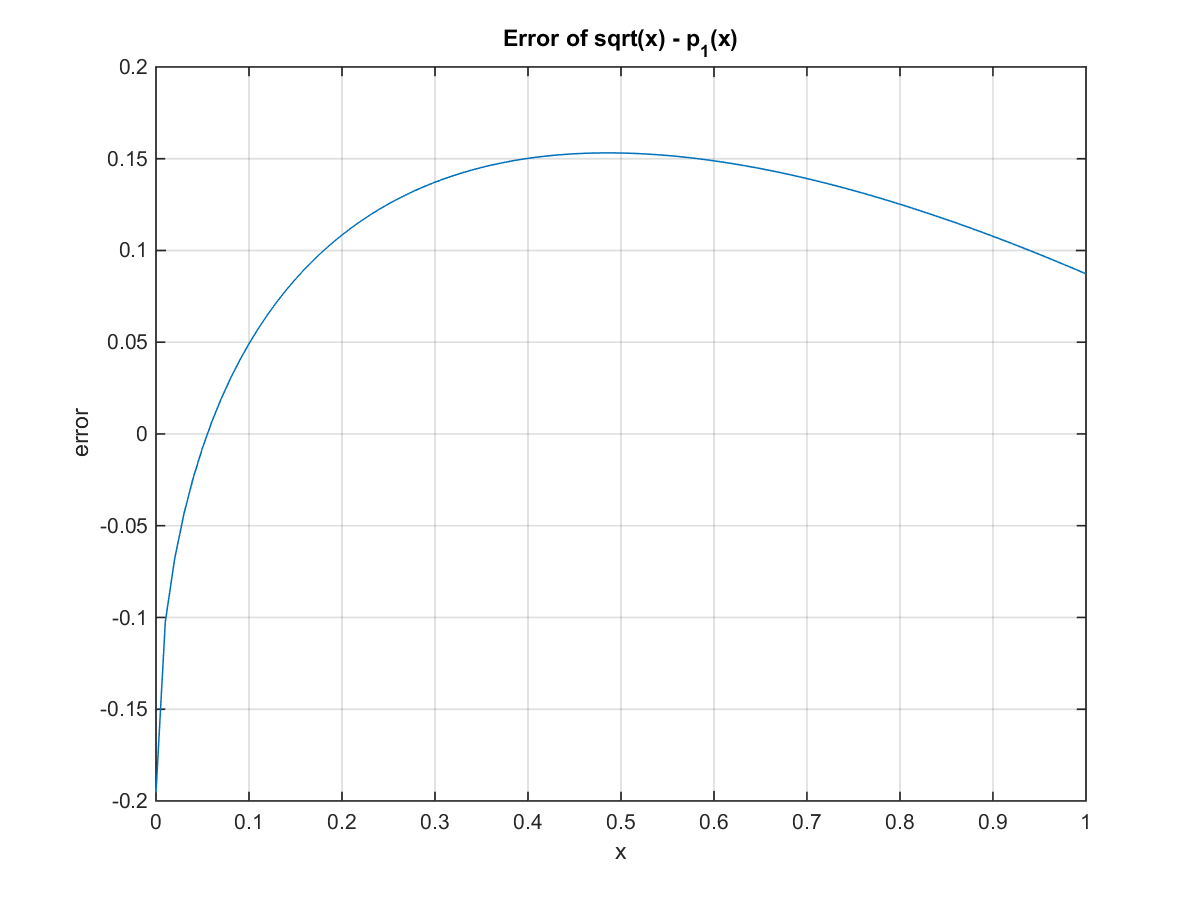
\includegraphics[scale =0.6]{hw3_11a.png}
		\caption{Error of $\sqrt{x} - p_1(x)$ over $[1/3, 2/3]$}
	\end{figure}
		
	Identify 3 points $\tilde{x}_0, \tilde{x}_1, \tilde{x}_2$, at which the error $f(x) - p_1(x)$ oscillates sign:\\
	Base on above figure, we could point out three oscillates points:\\ 
	\hspace*{2cm} $\tilde{x}_0 = 0.2, \tilde{x}_1 = 0.5, \tilde{x}_2 = 0.8$ \\
		Apply \textbf{\textit{de la Valee Poussin}}'s theorem:\\
	$\|f-p_*\|_{\infty} \geq \min\limits_{0\leq j \leq n+1} |f(x_j) - p_1(x_j)| = \min\limits_{0\leq x_j \leq 1} \left|\sqrt{x} - (\sqrt{6} - \sqrt{3})x - \dfrac{2 -\sqrt{2}}{\sqrt{3}} \right|$\\
	For error function: $e(x) = \sqrt{x} - (\sqrt{6} - \sqrt{3})x - \dfrac{2 -\sqrt{2}}{\sqrt{3}}$\\
	\hspace*{3.4cm} $ e'(x) = \dfrac{1}{2\sqrt{x}} - (\sqrt{6}-\sqrt{3})$ \\
	so that $ e'(x) = 0 \Leftrightarrow x = \dfrac{1}{4(9-6\sqrt{2})} = 0.4857$\\
	$\Rightarrow \min\limits_{0\leq x_j \leq 1}|e(x)| = \left. \left|\sqrt{x} - (\sqrt{6} - \sqrt{3})x - \dfrac{2 -\sqrt{2}}{\sqrt{3}} \right| \right|_{x = 0.4857} = 0.0103 $ \\
	
	The lower bound on the error: $\|f-p_*\|_{\infty} \geq 0.0103$
	
	\label{1b}
	\item For the same interpolant $p_1$ at $x_0 = 1/3$ and $x_2 = 2/3$, Problem 3 of Problem set 2 gives a different lower bound on $\|f-p_*\|_{\infty}$:\\
	\hspace*{5cm} $\dfrac{\|f-p_1\|_{\infty}}{1 + \|\Pi_1\|_{\infty}} \leq \|f-p_*\|_{\infty}$ \\
	Compute (by hand) the left hand side:\\
	We first have: $\|f-p_1\|_{\infty} = \min\limits_{x\in [0,1]}\left| \sqrt{x} - \left( \sqrt{6}-\sqrt{3}\right)x - \dfrac{2 - \sqrt{2}}{\sqrt{3}} \right| = 0.0103$\\
	After that: $\|\Pi_1\|_{\infty} = \max\limits_{x \in [0,1]} |l_0(x)| + |l_1(x)|$\\
	$$ l_0(x) = \prod_{k=0,k\neq 0}^{1} \dfrac{x - x_k}{x_0-x_k} = \dfrac{x - x_1}{x_0 - x_1} = \dfrac{x - \frac{2}{3}}{\frac{1}{3} - \frac{2}{3}} = -3\left(x - \frac{2}{3} \right) = 2 - 3x $$
	$$ l_1(x) = \prod_{k=0,k\neq 1}^{1} \dfrac{x - x_k}{x_1-x_k} = \dfrac{x - x_0}{x_1 - x_0} = \dfrac{x - \frac{1}{3}}{\frac{2}{3} - \frac{1}{3}} = 3\left(x - \frac{1}{3} \right) = 3x-1 $$  
	$\Rightarrow \|\Pi_1\|_{\infty} = \max\limits_{x \in [0,1]} |l_0(x)| + |l_1(x)| = \max\limits_{x \in [0,1]} \left( |2-3x| + |3x-1|\right) = 3$\\
	So that: $\dfrac{\|f-p_1\|_{\infty}}{1 + \|\Pi_1\|_{\infty}} = \dfrac{0.0103}{1+3} = 0.002575$\\
	
	\label{1c}
	\item Now compute $p_* \in \mathcal{P}_1$ that best approximates $\sqrt{x}$ in the minimax sense, and report the error. Is this error consistent with the bounds you obtained in part (a)? [Kincaid \& Cheney]\\
	For minimax sense: $p_*(x) = \alpha + \beta x \in \mathcal{P}_1$ with $x_0 = 0, x_2=1$:\\
	$\begin{cases} \delta = f(x_0) - (\alpha + \beta x_0) \\ -\delta = f(x_1) - (\alpha + \beta x_1) \\ \delta = f(x_2) - (\alpha + \beta x_2) \\ f'(x_1) - p'_*(x_1) = 0  \end{cases} \Leftrightarrow \begin{cases} \delta = 0 - (\alpha + \beta .0) \\ -\delta = \sqrt{x_1} - (\alpha + \beta x_1) \\ \delta = 1 - (\alpha + \beta .1) \\ \dfrac{1}{2\sqrt{x_1}} = \beta \end{cases} \Leftrightarrow \begin{cases} \alpha = \dfrac{1}{8} \\ \beta = 1 \\ \delta = -\dfrac{1}{8} \\ x_1 = \dfrac{1}{4} \end{cases}$ \\
	So we have: $p_* = \dfrac{1}{8} + x$\\
	The error is presented in following figure:
	\begin{figure}[htp]
		\centering
		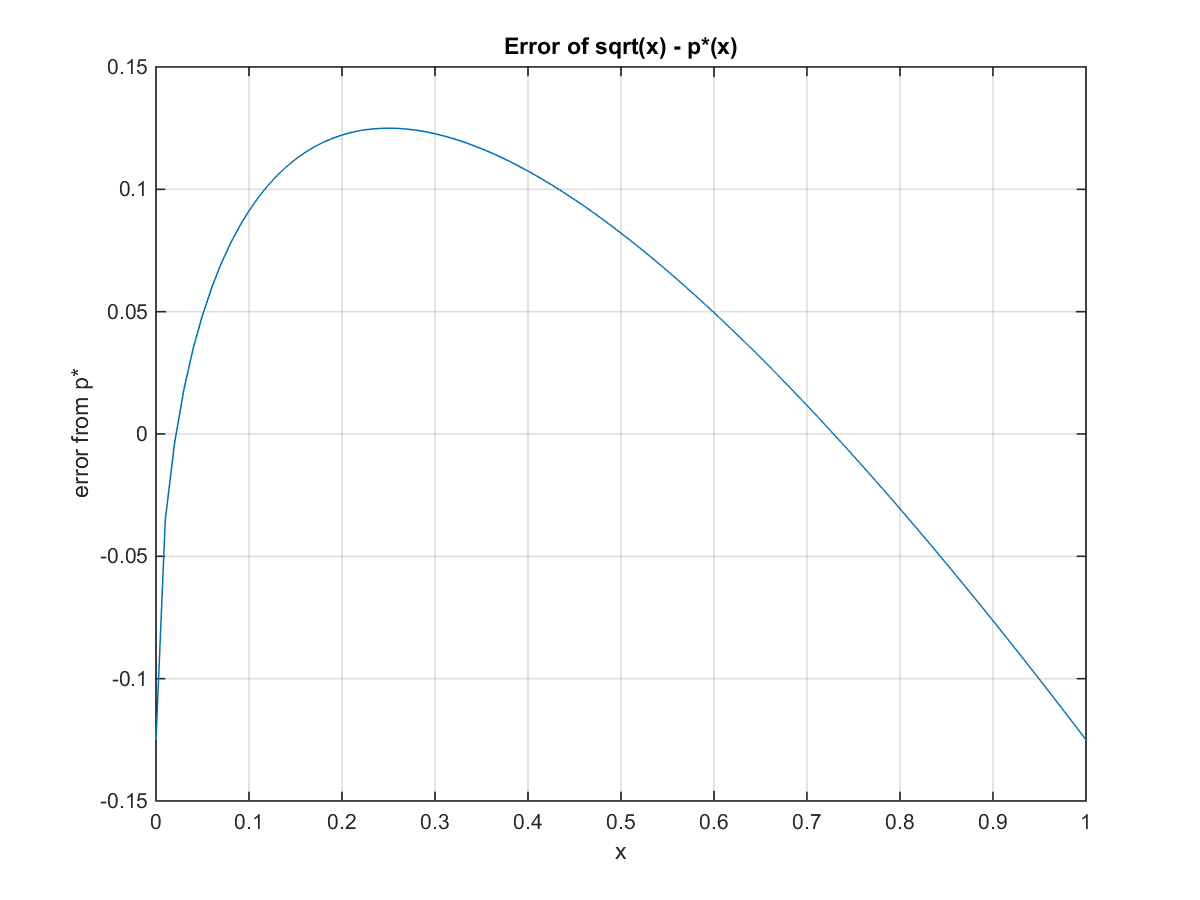
\includegraphics[scale=0.7]{hw3_11c.png}
		\caption{Error of $p_*$ approximation}
	\end{figure}\\
	The error is bounded by: $\min\|f-p_*\|_{\infty} = \dfrac{1}{8}$ at $x=x_1= \dfrac{1}{4}$\\
	From that we see: $\dfrac{1}{8} = 0.125 >> 0.0103 \Rightarrow $ so the error is consistent with the bounds obtained from part (a).\\
\end{enumerate}
\pagebreak

\label{Problem 2}
\large\textbf{Problem 2.} 
\begin{enumerate}
	\label{2a} 
	\item Find the line $P_* \in \mathcal{P}_1$ that gives a least square approximation to $f(x) = \sqrt{x}$ on $x \in [0,1]$, and report the error $\|f-P_*\|_2$\\
	We have the form of $P_*$: $P_* = P_1 = c_0\Phi_0 + c_1\Phi_1$ with $\begin{cases} \Phi_0 = x^0 = 1 \\ \Phi_1 = x^1 = x \end{cases}$ \\
	So: $P_* = c_0 + c_1x$, so that we form the following equation: \\
	\hspace*{2cm} $\begin{bmatrix} \langle\Phi_0,\Phi_0\rangle & \langle\Phi_0,\Phi_1\rangle \\ \langle\Phi_1,\Phi_0\rangle & \langle\Phi_1,\Phi_1\rangle \end{bmatrix} \begin{bmatrix} c_0\\c_1 \end{bmatrix}  = \begin{bmatrix} \langle f,\Phi_0\rangle \\ \langle f,\Phi_1\rangle \end{bmatrix}  $ \\
	with: $$ \langle\Phi_0,\Phi_0\rangle = \langle 1,1 \rangle = \int_{0}^{1}1.1.\mathrm{d}x = \left. x\right|_0^1 = 1$$
	$$ \langle\Phi_0,\Phi_1\rangle = \langle\Phi_1,\Phi_0\rangle = \langle 1,x \rangle = \int_{0}^{1}1.x.\mathrm{d}x = \left.\dfrac{1}{2} x^2\right|_0^1 = \dfrac{1}{2}$$
	$$ \langle\Phi_1,\Phi_1\rangle = \langle x,x \rangle = \int_{0}^{1}x.x\mathrm{d}x = \left. \dfrac{1}{3}x^3\right|_0^1 = \dfrac{1}{3}$$
	$$ \langle f,\Phi_0 \rangle = \langle x^{\frac{1}{2}},1 \rangle = \int_{0}^{1}x^{\frac{1}{2}}.1.\mathrm{d}x = \left.\dfrac{x^{\frac{3}{2}}}{\frac{3}{2}}\right|_0^1 = \dfrac{2}{3} $$ 
	$$ \langle f,\Phi_1 \rangle = \langle x^{\frac{1}{2}},x \rangle = \int_{0}^{1}x^{\frac{1}{2}}.x.\mathrm{d}x = \left.\dfrac{x^{\frac{5}{2}}}{\frac{5}{2}}\right|_0^1 = \dfrac{2}{5} $$ 
	So: $\begin{bmatrix} 1& \frac{1}{2} \\ \frac{1}{2} & \frac{1}{3} \end{bmatrix} \begin{bmatrix} c_0\\c_1 \end{bmatrix} = \begin{bmatrix} \frac{2}{3} \\ \frac{2}{5} \end{bmatrix} \Leftrightarrow \begin{cases} c_0 = \dfrac{4}{15} \\ c_1 = \dfrac{4}{5} \end{cases} $ \\
	$\Rightarrow P_* = \dfrac{4}{15} + \dfrac{4}{5}x $\\
	The error is presented as bellow (figure 3):
	\begin{figure}[htp]
		\centering
		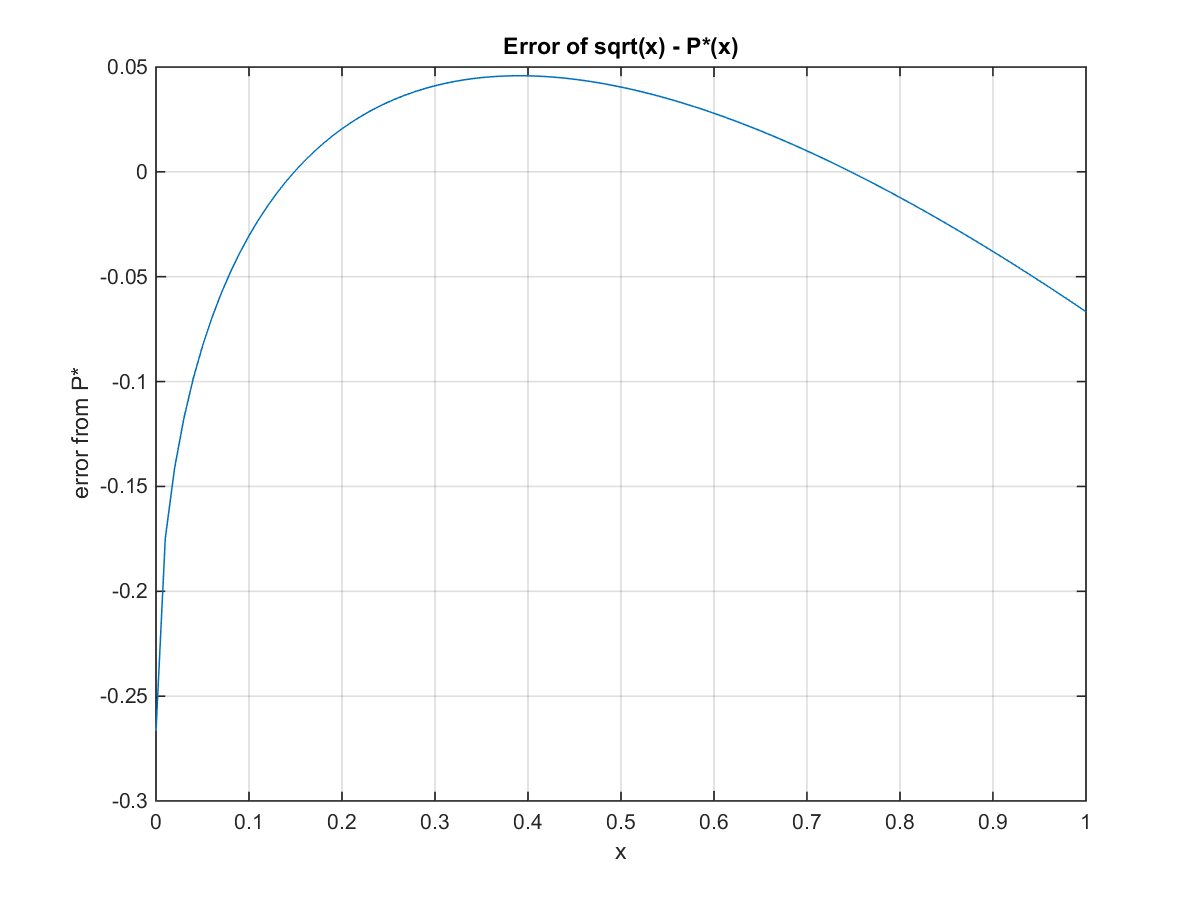
\includegraphics[scale=0.7]{hw3_21a.png}
		\caption{Error of $P_*$ approximation}
	\end{figure}
	
	\label{2b}	
	\item For a general interval $[a,b]$, prove that for all $f \in C[a,b]$: \\
	\hspace*{5cm} $ \min\limits_{p \in \mathcal{P}_n} \|f-p\|_2 \leq \sqrt{b-a} \min\limits_{p \in \mathcal{P}_n}\|f-p\|_{\infty}$\\
	We have: $\min\limits_{p \in \mathcal{P}_n} \|f-p\|_2 = \|f-p_*\|_2$ and $\min\limits_{p \in \mathcal{P}_n} \|f-p\|_{\infty} = \|f-p_*\|_{\infty}$\\
	\hspace*{3cm} and $|f-p_*| \leq \|f-p_*\|_{\infty}$\\
	Based on Example 8.2 \{S$u$li and Mayers\} equation:\\ $$\|f\|_2 = \left( \int_{a}^{b}w(x)|f(x)|^2\mathrm{d}x \right)^{\frac{1}{2}}$$
	Applied above equation with the \textbf{\textit{weight function $w(x) = 1$}} we have:
	$$\|f-p_*\|_2 = \left( \int_{a}^{b}w(x)|f(x)-p_*(x)|^2\mathrm{d}x \right)^{\frac{1}{2}} \leq \left( \int_{a}^{b}1.\left(\|f(x)-p_*(x)\|_{\infty}\right)^2\mathrm{d}x \right)^{\frac{1}{2}} $$
	$$ \Leftrightarrow \|f-p_*\|_2 \leq \left( \int_{a}^{b}1.\mathrm{d}x \int_{a}^{b}\left(\|f(x)-p_*(x)\|\right)^2\mathrm{d}x \right)^{\frac{1}{2}}$$
	 $$ \Leftrightarrow \|f-p_*\|_2 \leq \left( \left.x\right|_a^b \right)^{\frac{1}{2}}.\left( \int_{a}^{b}\left(\|f(x)-p_*(x)\|_{\infty}\right)^2\mathrm{d}x \right)^{\frac{1}{2}}  $$
	$$ \Leftrightarrow \|f-p_*\|_2 \leq \sqrt{b-a}.\|f(x)-p_*(x)\|_{\infty}$$
	$$ \Leftrightarrow \min\limits_{p \in \mathcal{P}_n} \|f-p\|_2 \leq \sqrt{b-a} \min\limits_{p \in \mathcal{P}_n} \|f-p\|_{\infty} $$
	
	%Confirm that your solutions to Problem 1(c) and 2(a) are consistent with this bound.\\
	For problem 1c and 2a we have $a=0, b=1 \Rightarrow$ The lower bound is defined as:\\
	\hspace*{2cm} $\min\limits_{p \in \mathcal{P}_n} \|f-p\|_2 \leq \min\limits_{p \in \mathcal{P}_n} \|f-p\|_{\infty} $\\
	\hspace*{1cm} i. From part 1c: $\min\limits_{p \in \mathcal{P}_n} \|f-p\|_{\infty} = 0.125$\\
	\hspace*{1cm} ii. From part 2a: $\min\limits_{p \in \mathcal{P}_n} \|f-p\|_2 = 0.0458$\\
	We have: $0.125 > 0.0458 \Rightarrow$ these 2 problems are consistent with the bound.
	\pagebreak
	
	\label{2c}
	\item Let $[a,b]$ be any fixed interval. Given any $\epsilon > 0$, show that there exist some $f \in C[a,b]$ such that $\|f\|_2 \leq \epsilon$, while $\|f\|_{\infty} \geq \frac{1}{\epsilon}$ .\\
	Define: $f(x) = \dfrac{2\dfrac{1}{\epsilon}}{\sqrt{1+k^2(x-c)^2}}$\\
	with: $c = \dfrac{1}{2}(a+b)$ and $k$ is a constant to be determined ($k > 0$).\\
	We first have: $\|f\|_{\infty} = 2\dfrac{1}{\epsilon} \geq \dfrac{1}{\epsilon} $\\
	After that: $$\left(\|f(x)\|_{\infty}\right)^2 = \int_{a}^{b}|f(x)|^2\mathrm{d}x = \int_{a}^{b} \dfrac{\dfrac{4}{\epsilon^2}}{1+k^2(x-c)^2}\mathrm{d}x $$
	$$ \Leftrightarrow \left(\|f(x)\|_{\infty}\right)^2 = \dfrac{4}{k\epsilon^2}\left( tan^{-1}\frac{1}{2}k(b-a) - tan^{-1}\frac{1}{2}k(a-b)\right) \leq \dfrac{4\pi}{k\epsilon^2} $$
	$$ \Leftrightarrow \|f(x)\|_{\infty} \leq \dfrac{2\sqrt{\pi}}{\epsilon\sqrt{k}} \hspace{1cm} (\Rightarrow k \leq \pi)$$
	
	Applied above result:\\
	\hspace*{1cm} $\begin{cases} \|f\|_2 \leq \sqrt{b-a}\|f\|_{\infty} \\ \|f\|_2 \leq \epsilon \quad (required) \end{cases} \Leftrightarrow \epsilon \leq \sqrt{b-a}.\dfrac{2\sqrt{\pi}}{\epsilon\sqrt{k}} \Leftrightarrow k \leq \dfrac{4\pi(b-a)}{\epsilon^4}$\\
	With $k$ meet above conditions ($k \leq \pi$, and $ k \leq \dfrac{4\pi(b-a)}{\epsilon^4}$ ), function $f(x)$ is exist.\\
	
	% (This implies that there exists \textit{no} constaint \textit{M} such that $\|f\|_{\infty} \leq M\|f\|_2$ for all $f \in C[a,b]$.) [Suli and Mayers, problem 8.1]\\
	
	
\end{enumerate}

\label{Problem 3}
\large\textbf{Problem 3.} Suppose we have a function $f \in C[a,b]$ but $f(x)$ is unbounded as $x \rightarrow a$. Then for any polynomial $p \in \mathcal{P}_n, \|f-p\|_{\infty}$ would be infinite over $[a,b]$, and hence there exists no minimax approximation. The last problem hints that the situation could possibly be better for least squares approximation. This problem, adapted from Gautchi, explores an example where this is the case.\\
The \textit{shifted Legendre polynomials} for the interval $x \in [0,1]$ are defined as $\pi_0(x)= 1, \pi_1(x) = 2x -1$, and then, for $n \geq 1$, via the recurrence:\\
\hspace*{4cm} $\pi_{n+1} = \dfrac{2n+1}{n+1} (2x-1)\pi_n(x) - \dfrac{n}{n+1}\pi_{n-1}(x)$\\
You may use without proof that these polynomial are \textit{orthogonal} with respect to inner product (and norm):\\
\hspace*{4cm} $\langle f,g\rangle = \int_{0}^{1} f(x)g(x)dx$, \hspace{1cm} $\|f\|_2 = (f,f)^{1/2}$\\
By longstanding convention these polynomials are constructed such that $\pi_n(1) =1$, so they are not \textit{orthonormal}. You may thus also use without proof that:\\
\hspace*{5cm} $ \left( \pi_j,\pi_j\right) = \dfrac{1}{2j+1}$\\
\begin{enumerate}
	\label{3a}
	\item Work out explicit formulas for $\pi_2(x)$ and $\pi_3(x)$; simplify as much as possible.\\
	- For n=1: $\pi_2(x) = \pi_{1+1}(x) = \dfrac{2*1+1}{1+1} (2x-1)\pi_1(x) - \dfrac{1}{1+1}\pi_0(x)$\\ 
	\hspace*{5cm} $ = \dfrac{3}{2}(2x-1)(2x-1) - \dfrac{1}{2}.1$\\
	\hspace*{5cm} $ = 6x^2 - 6x +1$\\
	- For n=2: $\pi_3(x) = \pi_{2+1}(x) = \dfrac{2*2+1}{2+1}(2x-1)\pi_2(x) - \dfrac{2}{2+1}\pi_1(x)$\\ 
	\hspace*{4.9cm} $ = \dfrac{5}{3}(2x-1)(6x^2 -6x+1) - \dfrac{2}{3}.(2x-1)$\\
	\hspace*{4.9cm} $ = 20x^3 -30x^2 + 12x -1$\\
	
	\label{3b}	
	We wish to approximate the \textit{unbounded} function $f(x)= log(1/x)$ (log denotes the natural logarithm).We will use these orthogonal polynomials as a basis for least squares approximation with degree-\textit{n} polynomials, writing the optimal polynomial $P_{*,n} \in \mathcal{P}$ in the form:
	\hspace*{5cm} $$ P_{*,n}(x) = \sum_{j=0}^{n} c_j\pi_j(x)$$
	\item Use the fact that: $$ \int_{0}^{1}\pi_j\log(1/x)\mathrm{d}x = \begin{cases} 1 \quad j = 0\\ \dfrac{(-1)^j}{j(j+1)} \quad j \geq 1 \end{cases} $$
	to determine formulas for the coefficient $c_0, ..., c_n$ in the best approximation\\
	The error based on least square approximation: $$ \|f-P_{*,n}\|_2 = \left( \int_{0}^{1}\left(f(x)-P_{*,n}(x)\right)^2\mathrm{d}x\right)^{\frac{1}{2}} = \left( \int_{0}^{1}\left(\log(\frac{1}{x})-\sum_{j=0}^{n} c_j\pi_j(x)\right)^2\mathrm{d}x\right)^{\frac{1}{2}} $$
	Define the Error function: $$E(c_0,c_1, ...,c_n) = \int_{0}^{1}\left(\log(\frac{1}{x})-\sum_{j=0}^{n} c_j\pi_j(x)\right)^2\mathrm{d}x $$
	 $$\Leftrightarrow E(c_0,c_1,...,c_n) = \|f\|^2 - 2\sum_{k=0}^{n}c_k\langle\log(\frac{1}{x}),\pi_k\rangle + \sum_{j=0}^{n}\sum_{k=0}^{n}c_jc_k\langle\pi_j,\pi_k\rangle $$
	Taking derivative of above equation for $c_0,c_1,...,c_n$ respectively, we have:
	$$ \sum_{j=0}^{n}c_j\langle\pi_j,\pi_l\rangle = \langle\log(\frac{1}{x}),\pi_l\rangle \hspace{1cm} l = 0,...,n$$
	Linear equation for coefficient $c_j$ is formed:\\
	\hspace*{1cm} $\begin{bmatrix} \langle\pi_0,\pi_0\rangle & \langle\pi_1,\pi_0\rangle &...&...&...& \langle\pi_n,\pi_0\rangle \\ \langle\pi_0,\pi_1\rangle & \langle\pi_1,\pi_1\rangle &...&...&...& \langle\pi_n,\pi_1\rangle \\ ...&...&...&...&...&... \\ \langle\pi_0,\pi_j\rangle & \langle\pi_1,\pi_j\rangle &...&...&...& \langle\pi_n,\pi_j\rangle \\ ...&...&...&...&...&... \\ \langle\pi_0,\pi_n\rangle & \langle\pi_1,\pi_n\rangle &...&...&...& \langle\pi_n,\pi_n\rangle \end{bmatrix}  \begin{bmatrix} c_0 \\ c_1 \\ ...\\c_j\\... \\c_n \end{bmatrix} = \begin{bmatrix} \langle\log(\frac{1}{x}),\pi_0\rangle \\ \langle\log(\frac{1}{x}),\pi_1\rangle \\ ... \\\langle\log(\frac{1}{x}),\pi_j\rangle \\ ...\\ \langle\log(\frac{1}{x}),\pi_n\rangle \end{bmatrix} $\\
	We can easily see that: $$\langle\pi_j,\pi_k\rangle = \int_{0}^{1}\pi_j(x)\pi_k(x)\mathrm{d}x= 0 \hspace{1.3cm}  for \hspace{0.2cm} j\neq k$$
	%Apply both:
	$$ \left( \pi_j,\pi_j\right) = \dfrac{1}{2j+1} \hspace{0.5cm} and \hspace{0.5cm} \int_{0}^{1}\pi_j\log(1/x)\mathrm{d}x = \begin{cases} 1 \quad j = 0\\ \dfrac{(-1)^j}{j(j+1)} \quad j \geq 1 \end{cases} $$
	Linear equation for coefficient $c_j$ is defined as:\\
	\hspace*{2cm} $\begin{bmatrix} 1&0&0&0&0&0 \\ 0& \dfrac{1}{3}&0&0&0&0 \\ ...&...&...&...&...&...\\0&0&0& \dfrac{1}{2j+1}&0&0\\...&...&...&...&...&...\\ 0&0&0&0&0& \dfrac{1}{2n+1}\end{bmatrix} \begin{bmatrix} c_0 \\ c_1 \\ ...\\c_j\\... \\c_n \end{bmatrix} = \begin{bmatrix} 1\\ -\dfrac{1}{2} \\ ...\\ \dfrac{(-1)^j}{j(j+1)}\\...\\\dfrac{(-1)^n}{n(n+1)} \end{bmatrix} $\\
	
	
	\label{3c}
	\item Prove that $\|f-P_{*,n}\| = \dfrac{1}{n+1}$ (Hint: use induction)\\
	We have: $$\|f-P_{*,n}\|^2 = \|f\|^2 - \|P_{*,n}\|^2 = \|f\|^2 - \sum_{k=0}^{n}\dfrac{\langle f,\pi_k\rangle^2}{\langle\pi_k,\pi_k\rangle} \hspace{1cm} (*)$$
	Assume that $x = e^{-t}$ we have:
	$$ \|f\|^2 = \int_{0}^{1}\left[\log(1/x)\right]^2\mathrm{d}x = \int_{\infty}^{0}t^2(-e^{-t})\mathrm{d}x = \int_{0}^{\infty}t^2e^{-t}\mathrm{d}x = 2! =2 $$
	Utilize the fact given in part (b):
	$$ \langle\pi_j,f\rangle =  \int_{0}^{1}\pi_j\log(1/x)\mathrm{d}x = \begin{cases} 1 \quad j = 0\\ \dfrac{(-1)^j}{j(j+1)} \quad j \geq 1 \end{cases} \Rightarrow \langle\pi_j,f\rangle^2 = \begin{cases} 1 \quad j = 0\\ \dfrac{1}{j^2(j+1)^2} \quad j \geq 1 \end{cases} $$
	Besides, from question's data: $ \langle\pi_j,\pi_j\rangle = \dfrac{1}{2j+1}$\\
	Replaced to (*) we have final result:
	$$\|f-P_{*,n}\|^2 = 2 - 1 - \sum_{j=1}^{n}\dfrac{\frac{1}{j^2(j+1)^2}}{\frac{1}{2j+1}} = 1 - \sum_{j=1}^{n}\dfrac{2j+1}{j^2(j+1)^2}$$
	$$ \Leftrightarrow \|f-P_{*,n}\|^2 = 1 - \sum_{j=1}^{n}\dfrac{(j+1)^2 - j^2}{j^2(j+1)^2} = 1 - \sum_{j=1}^{n}\dfrac{1}{j^2} + \sum_{j=1}^{n}\dfrac{1}{(j+1)^2} $$
	$$ \Leftrightarrow \|f-P_{*,n}\|^2 = 1 - \sum_{j=1}^{n}\dfrac{1}{j^2} + \sum_{j=2}^{n+1}\dfrac{1}{j^2} = 1 - 1 + \dfrac{1}{(n+1)^2} = \dfrac{1}{(n+1)^2}$$
	So that: $  \|f-P_{*,n}\| = \dfrac{1}{n+1}$
	\pagebreak
	
	\label{3d}
	\item Create a plot comparing $f$ to the first four least squares approximation: $P_{*,0}, P_{*,1}, P_{*,2}, P_{*,3}$.\\
	For $n=3$ we have the specific linear equation for coefficient $c_j$:\\
	\hspace*{2cm} $\begin{bmatrix} 1&0&0&0 \\ 0&\dfrac{1}{3}&0&0 \\0&0&\dfrac{1}{5}&0 \\0&0&0&\dfrac{1}{7} \end{bmatrix} \begin{bmatrix} c_0\\c_1\\c_2\\c_3 \end{bmatrix} = \begin{bmatrix} 1\\-\dfrac{1}{2} \\ \dfrac{1}{6} \\ -\dfrac{1}{12} \end{bmatrix} \Leftrightarrow \begin{cases} c_0 = 1 \\ c_1 = -\dfrac{3}{2} \\ c_2 = \dfrac{5}{6} \\ c_3 = -\dfrac{7}{12} \end{cases} $ \\
	The first four least square approximation is defined:\\
	$P_{*,0} = c_0\pi_0 = 1.1 = 1$\\
	$P_{*,1} = c_0\pi_0 + c_1\pi_1 = 1.1 - \dfrac{3}{2}(2x-1) = -3x + \dfrac{5}{2}$\\
	$P_{*,2} = c_0\pi_0 + c_1\pi_1 + c_2\pi_2 = 1.1 - \dfrac{3}{2}(2x-1) + \dfrac{5}{6}(6x^2-6x+1) = 5x^2 -8x + \dfrac{10}{3}$\\
	$P_{*,3} = c_0\pi_0 + c_1\pi_1 + c_2\pi_2 + c_3\pi_3$\\
	\hspace*{0.7cm} $ = 1.1 - \dfrac{3}{2}(2x-1) + \dfrac{5}{6}(6x^2-6x+1) - \dfrac{7}{12}(20x^3 -30x^2 + 12x -1)$ \\
	\hspace*{0.7cm} $ = - \dfrac{35}{3}x^3 + \dfrac{45}{2}x^2 -15x + \dfrac{47}{12}$\\
	Approximations are presented in following plot:\\
	\begin{figure}[htp]
		\centering
		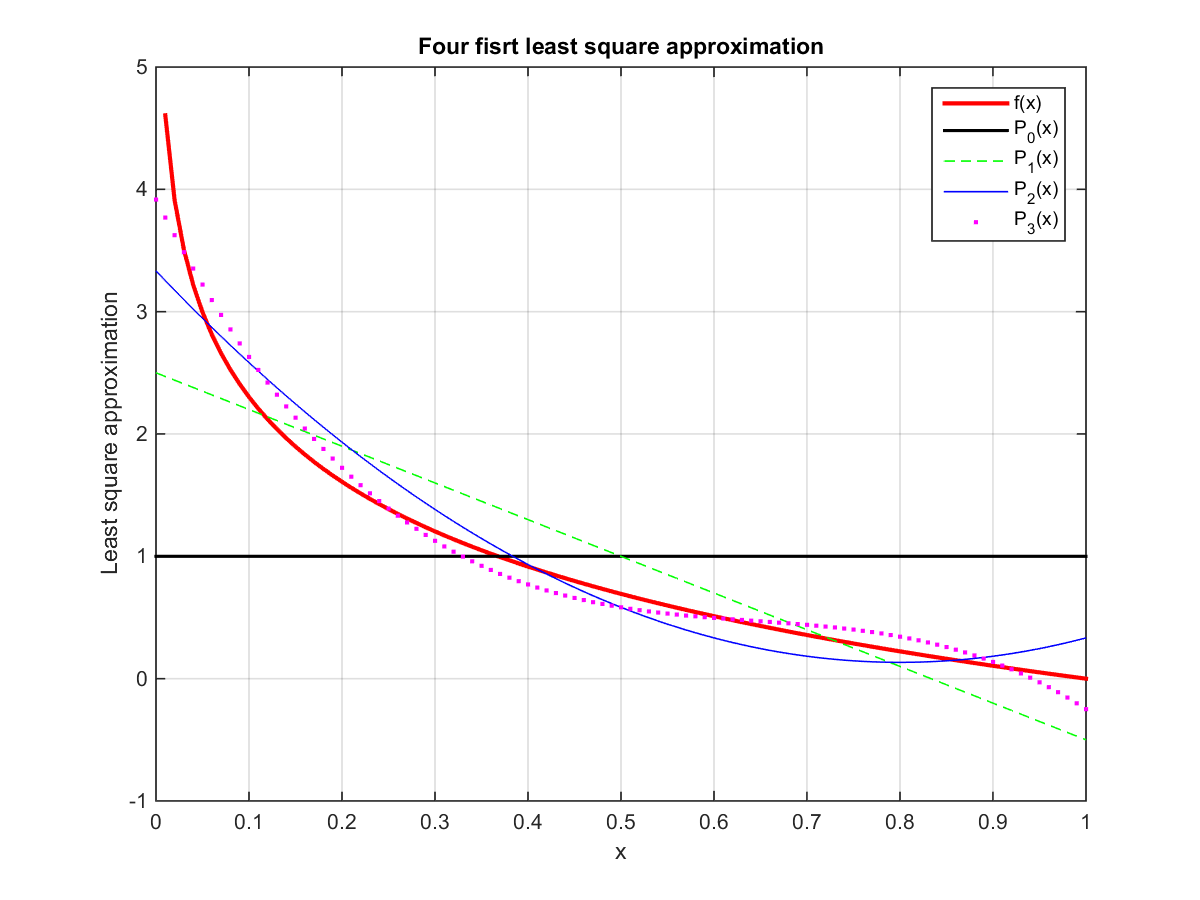
\includegraphics[scale=0.7]{hw3_34.png}
		\caption{First four least square approximation of $f(x) = \log(\dfrac{1}{x})$}
	\end{figure}
\end{enumerate}

\label{Problem 4}
\large\textbf{Problem 4.} The \textit{conjugate gradient algorithm} is the most important iterative method for solving the linear system of equations $\textbf{Ac} = \textbf{b}$ when the matrix $\textbf{A} \in \mathbb{R}^{NxN}$ is large, sparse, and symmetric positive define. Since \textbf{A} is symmetric positive definite, its eigenvalues are real and positive; write them as: $0 < \lambda_1 \leq \lambda_2 \leq ... \leq \lambda_N$\\ 
One can show that at step $k$, the conjugate gradient algorithm constructs an iterate $\textbf{c}_k$ such that:\\
\hspace*{4cm} $ \dfrac{\|\textbf{c} - \textbf{c}_k\|_{\textbf{A}}}{\|\textbf{b}\|_{\textbf{A}}} \leq \min\limits_{p \in \mathcal{P}_k,p(0) =1} \max\limits_{x\in[\lambda_1,\lambda_N]} |p(x)|$\\
(Here $\|.\|_{\textbf{A}}$ defines the \textit{energy norm} induced by \textbf{A}: $\|z\|_{\textbf{A}} = (z^T\textbf{A}z)^{1/2}$.)
\begin{enumerate}
	\label{4a}
	\item Derive the solution to the problem: \hspace{0.3cm} $ \min\limits_{p \in \mathcal{P}_k,p(0) =1} \max\limits_{x\in[\lambda_1,\lambda_N]} |p(x)|$\\
	in term of Chebyshev polynomials.\\
	Chebyshev polynomials is defined by: $T_n(x) = \cos(n\cos^{-1}x)$ for $x \in [-1,1]$\\
	$n = 0$: $T_0(x) = \cos(0\cos^{-1}x) = \cos(0) = 1$\\
	$n = 1$: $T_1(x) = \cos(1\cos^{-1}x) = x$\\
	$n = 2$: $T_2(x) = \cos(2\cos^{-1}x) = 2\cos^2(\cos^{-1}x) - 1 = 2x^2 -1$\\
	In general, for $n \geq 2$: $T_{n+1}(x) = 2xT_n(x) - T_{n-1}(x)$\\
	We also can represent Chebyshev polynomial by:\\
	\hspace*{3cm} $T_n(x) = \dfrac{1}{2}\left[(x+\sqrt{x^2-1})^n + (x - \sqrt{x^2-1})^n\right]$\\
	so if $x = x_j = \cos(\dfrac{n\pi}{n})$ then $T_n(x_j) = (-1)^n$, $j = 0,1,...n$\\
	Define a polynomial $q_n$: $q_n(\lambda) = \left[ T_n\left(\dfrac{\lambda_N+\lambda_1}{\lambda_N-\lambda_1}\right)\right]^{-1}.T_n\left(\dfrac{\lambda_N + \lambda_1 - 2\lambda}{\lambda_N - \lambda_1}\right)$ \\
	because of $|T_n(x)| \leq 1$ for all $x \in [-1,1]$ so:\\
	\hspace*{4cm} $\max\limits_{\lambda \in [\lambda_1,\lambda_N]}|q_n| = \left|T_n\left(\dfrac{\lambda_N+\lambda_1}{\lambda_N-\lambda_1}\right)\right|^{-1} = t_*$ \\
	Let $\mu_j = \dfrac{\lambda_1 - \lambda_N}{2}x_j + \dfrac{\lambda_1 + \lambda_N}{2}$ with defined $x_j$ above, so:\\
	\hspace*{1cm} i. $p_n(\mu_j) = (-1)^jt_*$, $j = 0,..., n$\\
	\hspace*{1cm}  ii. $\mu_j \in [\lambda_1, \lambda_N]$\\
	Assume that there exists a polynomial $p_n \in \mathcal{P}_n$, which is the best approximation for $T_n(x)$ with $p_n(0) = 1$ and: $|p_n(\lambda)| < |t_*|$ for all $\lambda \in [\lambda_1, \lambda_N]$\\
	it means that: $-|t_*| < p_n(\mu_j) < |t_*|$ with $j = 0,...,n$\\
	If $sign(t_*) > 0$ then: $\begin{cases} p_n(\mu_j) - q_n(\mu_j) < 0 \quad for \hspace{0.2cm} m \hspace{0.2cm} even \\ p_n(\mu_j) - q_n(\mu_j) > 0 \quad for \hspace{0.2cm} m \hspace{0.2cm} odd \end{cases}$\\
	If $sign(t_*) < 0$ then: $\begin{cases} p_n(\mu_j) - q_n(\mu_j) < 0 \quad for \hspace{0.2cm} m \hspace{0.2cm} odd \\ p_n(\mu_j) - q_n(\mu_j) > 0 \quad for \hspace{0.2cm} m \hspace{0.2cm} even \end{cases}$\\
	Hence, regardless of the \texttt{sign} of $t_*$, the different $p_n - q_n$ has a zero in every interval $(\mu_j,\mu_{j+1})$. There are $n$ such intervals.\\
	But we also have that $p_n(0) - q_n(0) = 1-1 =0$. Since $p_n - q_n$ is a polynomial of degree $n$, so $p_n \equiv q_n$.\\
	As a result: $ \min\limits_{p \in \mathcal{P}_k,p(0) =1} \max\limits_{x\in[\lambda_1,\lambda_N]} |p(x)| = \min\limits_{p \in \mathcal{P}_k,p(0) =1} \max\limits_{x\in[\lambda_1,\lambda_N]} |q_n(x)| = \left|T_n\left(\dfrac{\lambda_N+\lambda_1}{\lambda_N-\lambda_1}\right)\right|^{-1}$\\
	
	\label{4b}	
	\item Write \texttt{MATLAB} routine \texttt{cheby.m} such that \texttt{Tkx = cheby(x,k)} evaluate $T_k(x)$
	\begin{lstlisting}
	function Tkx = cheby(x,k)
		Tkx = cos(k*acos(x));
	end
	\end{lstlisting}
	
	
	\label{4c}
	\item Plot the minimizing polynomial in part (a) for $k = 3$ and $k=5$ for:\\
	(i) $\lambda_1 = 1, \lambda_N = 4$
	\begin{figure}[htp]
		\centering
		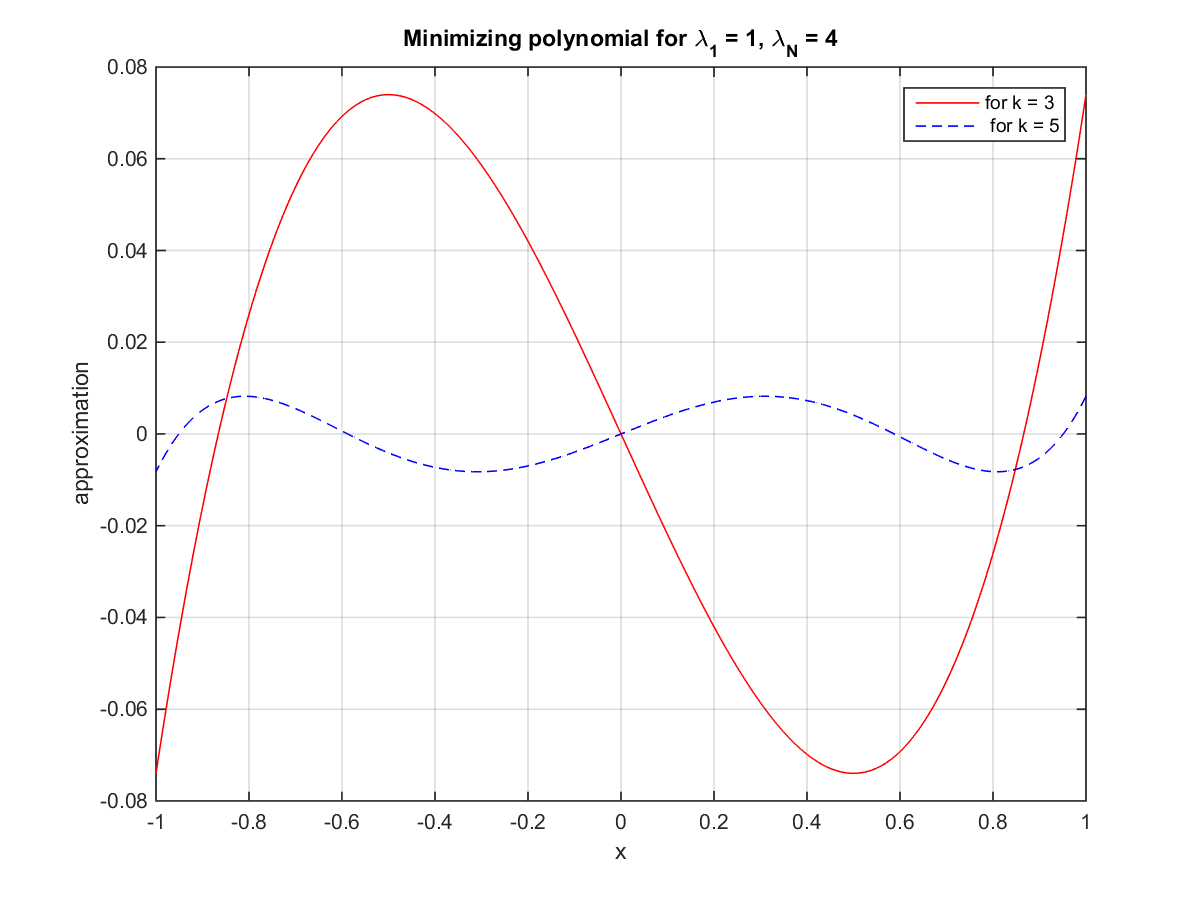
\includegraphics[scale=0.6]{hw3_414.png}
		\caption{Minimizing polynomial for $\lambda_1 = 1, \lambda_N = 4$}
	\end{figure}\\
	\pagebreak
	
	(ii) $\lambda_1 = 1, \lambda_N = 16$
	\begin{figure}[htp]
		\centering
		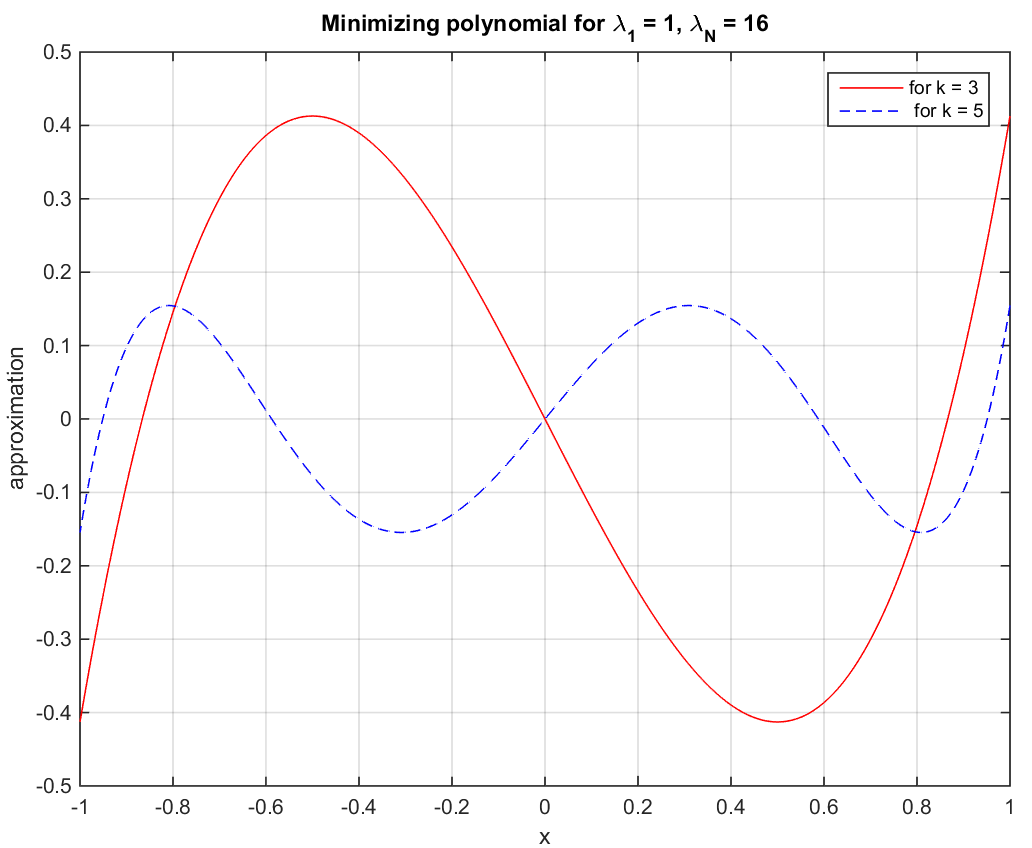
\includegraphics[scale=0.58]{hw3_4116.png}
		\caption{Minimizing polynomial for $\lambda_1 = 1, \lambda_N = 4$}
	\end{figure}\\
	(iii) $\lambda_1 = 1/4, \lambda_N = 4$
	\begin{figure}[htp]
		\centering
		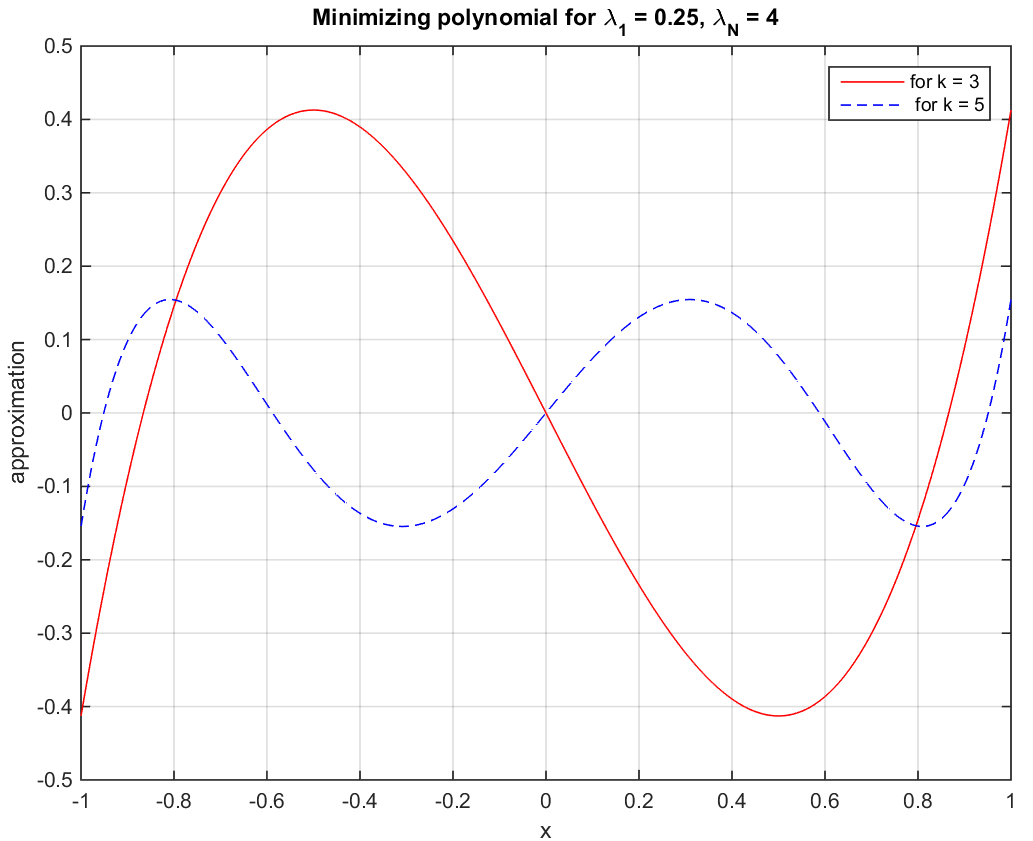
\includegraphics[scale=0.58]{hw3_43.png}
		\caption{Minimizing polynomial for $\lambda_1 = 1/4, \lambda_N = 4$}
	\end{figure}
	
	\label{4d}
	\item Use your answer from part (a) to derive the classic error bound for conjugate gradients:\\
	\hspace*{2.5cm} $ \min\limits_{p \in \mathcal{P}_k,p(0) =1} \max\limits_{x\in[\lambda_1,\lambda_N]} |p(x)| \leq 2\left( \dfrac{\sqrt{\lambda_N/\lambda_1}-1}{\sqrt{\lambda_N/\lambda_1}+1}\right)^k $\\
	For $x = \dfrac{\lambda_N + \lambda_1}{\lambda_N - \lambda_1} = \dfrac{\lambda_N/\lambda_1 +1}{\lambda_N/\lambda_1 -1}$, replaced into above equation we have:\\
	$x \pm \sqrt{x^2 -1} = \dfrac{\lambda_N/\lambda_1 +1}{\lambda_N/\lambda_1 -1} \pm \dfrac{2\sqrt{\lambda_N/\lambda_1}}{\lambda_N/\lambda_1 -1} = \dfrac{\lambda_N/\lambda_1 + 1 \pm 2\sqrt{\lambda_N/\lambda_1}}{\lambda_N/\lambda_1 -1}$\\
	\hspace*{7.2cm} $ = \dfrac{(\sqrt{\lambda_N/\lambda_1} \pm 1)^2}{(\sqrt{\lambda_N/\lambda_1}-1)(\sqrt{\lambda_N/\lambda_1}+1)}$\\
	\hspace*{7.2cm} $ = \dfrac{\sqrt{\lambda_N/\lambda_1} \pm 1}{\sqrt{\lambda_N/\lambda_1} \mp 1} $\\
	Thus: \\ 
	\hspace*{1cm} $T_n\left( \dfrac{\lambda_N + \lambda_1}{\lambda_N - \lambda_1} \right) = \dfrac{1}{2}\left[ \left(\dfrac{\sqrt{\lambda_N/\lambda_1}+1}{\sqrt{\lambda_N/\lambda_1} -1}\right)^n + \left(\dfrac{\sqrt{\lambda_N/\lambda_1}-1}{\sqrt{\lambda_N/\lambda_1} +1}\right)^n \right]$ \\
	Finally:\\
	\hspace*{1cm} $\left|T_n\left(\dfrac{\lambda_N+\lambda_1}{\lambda_N-\lambda_1}\right)\right|^{-1} = \dfrac{2}{\left(\dfrac{\sqrt{\lambda_N/\lambda_1}+1}{\sqrt{\lambda_N/\lambda_1} -1}\right)^n + \left(\dfrac{\sqrt{\lambda_N/\lambda_1}-1}{\sqrt{\lambda_N/\lambda_1} +1}\right)^n}$\\
	\hspace*{4.6cm} $\leq 2\left(\dfrac{\sqrt{\lambda_N/\lambda_1}-1}{\sqrt{\lambda_N/\lambda_1} +1}\right)^n $\\
	So: $ \min\limits_{p \in \mathcal{P}_k,p(0) =1} \max\limits_{x\in[\lambda_1,\lambda_N]} |p(x)| \leq 2\left( \dfrac{\sqrt{\lambda_N/\lambda_1}-1}{\sqrt{\lambda_N/\lambda_1}+1}\right)^k $ \hspace{1cm} \textbf{\textit{Proved!}}\\
	
	
	What kind of eigenvalue intervals $[\lambda_1,\lambda_N]$ lead the conjugate gradient algorithm to converge quickly? Slowly?\\
	\hspace*{1cm} \textbf{\textit{From above result we have:}}\\
	i. If $\lambda_N >> \lambda_1 \Rightarrow\left( \dfrac{\sqrt{\lambda_N/\lambda_1}-1}{\sqrt{\lambda_N/\lambda_1}+1}\right) $ is closer to 1 $\Rightarrow$ the upper bound is closer to 2 (get the maximum value) $\Rightarrow$ the conjugate gradient algorithm to converge is slow.\\
	ii. If $\lambda_N \approx \lambda_1 \Rightarrow\left( \dfrac{\sqrt{\lambda_N/\lambda_1}-1}{\sqrt{\lambda_N/\lambda_1}+1}\right) \approx 0 $ (closer to 0) $\Rightarrow$ the upper bound is closer to 0 (get the minimum value) $\Rightarrow$ the conjugate gradient algorithm to converge is fast.\\
	 
\end{enumerate}
	
	 
\end{document}